\documentclass[1p]{elsarticle_modified}
%\bibliographystyle{elsarticle-num}

%\usepackage[colorlinks]{hyperref}
%\usepackage{abbrmath_seonhwa} %\Abb, \Ascr, \Acal ,\Abf, \Afrak
\usepackage{amsfonts}
\usepackage{amssymb}
\usepackage{amsmath}
\usepackage{amsthm}
\usepackage{scalefnt}
\usepackage{amsbsy}
\usepackage{kotex}
\usepackage{caption}
\usepackage{subfig}
\usepackage{color}
\usepackage{graphicx}
\usepackage{xcolor} %% white, black, red, green, blue, cyan, magenta, yellow
\usepackage{float}
\usepackage{setspace}
\usepackage{hyperref}

\usepackage{tikz}
\usetikzlibrary{arrows}

\usepackage{multirow}
\usepackage{array} % fixed length table
\usepackage{hhline}

%%%%%%%%%%%%%%%%%%%%%
\makeatletter
\renewcommand*\env@matrix[1][\arraystretch]{%
	\edef\arraystretch{#1}%
	\hskip -\arraycolsep
	\let\@ifnextchar\new@ifnextchar
	\array{*\c@MaxMatrixCols c}}
\makeatother %https://tex.stackexchange.com/questions/14071/how-can-i-increase-the-line-spacing-in-a-matrix
%%%%%%%%%%%%%%%

\usepackage[normalem]{ulem}

\newcommand{\msout}[1]{\ifmmode\text{\sout{\ensuremath{#1}}}\else\sout{#1}\fi}
%SOURCE: \msout is \stkout macro in https://tex.stackexchange.com/questions/20609/strikeout-in-math-mode

\newcommand{\cancel}[1]{
	\ifmmode
	{\color{red}\msout{#1}}
	\else
	{\color{red}\sout{#1}}
	\fi
}

\newcommand{\add}[1]{
	{\color{blue}\uwave{#1}}
}

\newcommand{\replace}[2]{
	\ifmmode
	{\color{red}\msout{#1}}{\color{blue}\uwave{#2}}
	\else
	{\color{red}\sout{#1}}{\color{blue}\uwave{#2}}
	\fi
}

\newcommand{\Sol}{\mathcal{S}} %segment
\newcommand{\D}{D} %diagram
\newcommand{\A}{\mathcal{A}} %arc


%%%%%%%%%%%%%%%%%%%%%%%%%%%%%5 test

\def\sl{\operatorname{\textup{SL}}(2,\Cbb)}
\def\psl{\operatorname{\textup{PSL}}(2,\Cbb)}
\def\quan{\mkern 1mu \triangleright \mkern 1mu}

\theoremstyle{definition}
\newtheorem{thm}{Theorem}[section]
\newtheorem{prop}[thm]{Proposition}
\newtheorem{lem}[thm]{Lemma}
\newtheorem{ques}[thm]{Question}
\newtheorem{cor}[thm]{Corollary}
\newtheorem{defn}[thm]{Definition}
\newtheorem{exam}[thm]{Example}
\newtheorem{rmk}[thm]{Remark}
\newtheorem{alg}[thm]{Algorithm}

\newcommand{\I}{\sqrt{-1}}
\begin{document}

%\begin{frontmatter}
%
%\title{Boundary parabolic representations of knots up to 8 crossings}
%
%%% Group authors per affiliation:
%\author{Yunhi Cho} 
%\address{Department of Mathematics, University of Seoul, Seoul, Korea}
%\ead{yhcho@uos.ac.kr}
%
%
%\author{Seonhwa Kim} %\fnref{s_kim}}
%\address{Center for Geometry and Physics, Institute for Basic Science, Pohang, 37673, Korea}
%\ead{ryeona17@ibs.re.kr}
%
%\author{Hyuk Kim}
%\address{Department of Mathematical Sciences, Seoul National University, Seoul 08826, Korea}
%\ead{hyukkim@snu.ac.kr}
%
%\author{Seokbeom Yoon}
%\address{Department of Mathematical Sciences, Seoul National University, Seoul, 08826,  Korea}
%\ead{sbyoon15@snu.ac.kr}
%
%\begin{abstract}
%We find all boundary parabolic representation of knots up to 8 crossings.
%
%\end{abstract}
%\begin{keyword}
%    \MSC[2010] 57M25 
%\end{keyword}
%
%\end{frontmatter}

%\linenumbers
%\tableofcontents
%
\newcommand\colored[1]{\textcolor{white}{\rule[-0.35ex]{0.8em}{1.4ex}}\kern-0.8em\color{red} #1}%
%\newcommand\colored[1]{\textcolor{white}{ #1}\kern-2.17ex	\textcolor{white}{ #1}\kern-1.81ex	\textcolor{white}{ #1}\kern-2.15ex\color{red}#1	}

{\Large $\underline{12a_{0127}~(K12a_{0127})}$}

\setlength{\tabcolsep}{10pt}
\renewcommand{\arraystretch}{1.6}
\vspace{1cm}\begin{tabular}{m{100pt}>{\centering\arraybackslash}m{274pt}}
\multirow{5}{120pt}{
	\centering
	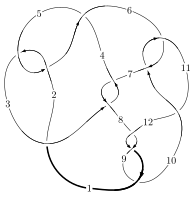
\includegraphics[width=112pt]{../../../GIT/diagram.site/Diagrams/png/928_12a_0127.png}\\
\ \ \ A knot diagram\footnotemark}&
\allowdisplaybreaks
\textbf{Linearized knot diagam} \\
\cline{2-2}
 &
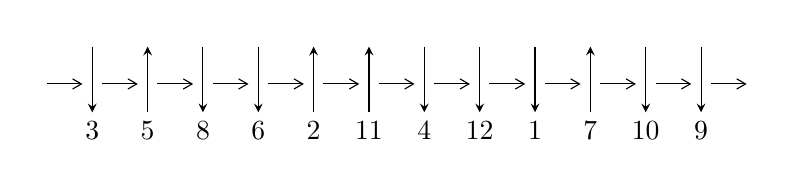
\begin{tikzpicture}[x=20pt, y=17pt]
	% nodes
	\node (C0) at (0, 0) {};
	\node (C1) at (1, 0) {};
	\node (C1U) at (1, +1) {};
	\node (C1D) at (1, -1) {3};

	\node (C2) at (2, 0) {};
	\node (C2U) at (2, +1) {};
	\node (C2D) at (2, -1) {5};

	\node (C3) at (3, 0) {};
	\node (C3U) at (3, +1) {};
	\node (C3D) at (3, -1) {8};

	\node (C4) at (4, 0) {};
	\node (C4U) at (4, +1) {};
	\node (C4D) at (4, -1) {6};

	\node (C5) at (5, 0) {};
	\node (C5U) at (5, +1) {};
	\node (C5D) at (5, -1) {2};

	\node (C6) at (6, 0) {};
	\node (C6U) at (6, +1) {};
	\node (C6D) at (6, -1) {11};

	\node (C7) at (7, 0) {};
	\node (C7U) at (7, +1) {};
	\node (C7D) at (7, -1) {4};

	\node (C8) at (8, 0) {};
	\node (C8U) at (8, +1) {};
	\node (C8D) at (8, -1) {12};

	\node (C9) at (9, 0) {};
	\node (C9U) at (9, +1) {};
	\node (C9D) at (9, -1) {1};

	\node (C10) at (10, 0) {};
	\node (C10U) at (10, +1) {};
	\node (C10D) at (10, -1) {7};

	\node (C11) at (11, 0) {};
	\node (C11U) at (11, +1) {};
	\node (C11D) at (11, -1) {10};

	\node (C12) at (12, 0) {};
	\node (C12U) at (12, +1) {};
	\node (C12D) at (12, -1) {9};
	\node (C13) at (13, 0) {};

	% arrows
	\draw[->,>={angle 60}]
	(C0) edge (C1) (C1) edge (C2) (C2) edge (C3) (C3) edge (C4) (C4) edge (C5) (C5) edge (C6) (C6) edge (C7) (C7) edge (C8) (C8) edge (C9) (C9) edge (C10) (C10) edge (C11) (C11) edge (C12) (C12) edge (C13) ;	\draw[->,>=stealth]
	(C1U) edge (C1D) (C2D) edge (C2U) (C3U) edge (C3D) (C4U) edge (C4D) (C5D) edge (C5U) (C6D) edge (C6U) (C7U) edge (C7D) (C8U) edge (C8D) (C9U) edge (C9D) (C10D) edge (C10U) (C11U) edge (C11D) (C12U) edge (C12D) ;
	\end{tikzpicture} \\
\hhline{~~} \\& 
\textbf{Solving Sequence} \\ \cline{2-2} 
 &
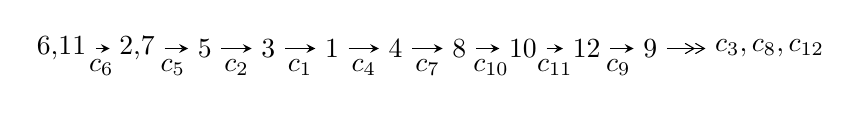
\begin{tikzpicture}[x=23pt, y=7pt]
	% node
	\node (A0) at (-1/8, 0) {6,11};
	\node (A1) at (17/16, 0) {2,7};
	\node (A2) at (17/8, 0) {5};
	\node (A3) at (25/8, 0) {3};
	\node (A4) at (33/8, 0) {1};
	\node (A5) at (41/8, 0) {4};
	\node (A6) at (49/8, 0) {8};
	\node (A7) at (57/8, 0) {10};
	\node (A8) at (65/8, 0) {12};
	\node (A9) at (73/8, 0) {9};
	\node (C1) at (1/2, -1) {$c_{6}$};
	\node (C2) at (13/8, -1) {$c_{5}$};
	\node (C3) at (21/8, -1) {$c_{2}$};
	\node (C4) at (29/8, -1) {$c_{1}$};
	\node (C5) at (37/8, -1) {$c_{4}$};
	\node (C6) at (45/8, -1) {$c_{7}$};
	\node (C7) at (53/8, -1) {$c_{10}$};
	\node (C8) at (61/8, -1) {$c_{11}$};
	\node (C9) at (69/8, -1) {$c_{9}$};
	\node (A10) at (11, 0) {$c_{3},c_{8},c_{12}$};

	% edge
	\draw[->,>=stealth]	
	(A0) edge (A1) (A1) edge (A2) (A2) edge (A3) (A3) edge (A4) (A4) edge (A5) (A5) edge (A6) (A6) edge (A7) (A7) edge (A8) (A8) edge (A9) ;
	\draw[->>,>={angle 60}]	
	(A9) edge (A10);
\end{tikzpicture} \\ 

\end{tabular} \\

\footnotetext{
The image of knot diagram is generated by the software ``\textbf{Draw programme}" developed by Andrew Bartholomew(\url{http://www.layer8.co.uk/maths/draw/index.htm\#Running-draw}), where we modified some parts for our purpose(\url{https://github.com/CATsTAILs/LinksPainter}).
}\phantom \\ \newline 
\centering \textbf{Ideals for irreducible components\footnotemark of $X_{\text{par}}$} 
 
\begin{align*}
I^u_{1}&=\langle 
-2.45704\times10^{149} u^{92}-7.46621\times10^{149} u^{91}+\cdots+1.59160\times10^{150} b+5.16311\times10^{150},\\
\phantom{I^u_{1}}&\phantom{= \langle  }6.45956\times10^{149} u^{92}+4.93708\times10^{149} u^{91}+\cdots+3.18320\times10^{150} a+3.19913\times10^{151},\\
\phantom{I^u_{1}}&\phantom{= \langle  }u^{93}+3 u^{92}+\cdots-120 u-16\rangle \\
I^u_{2}&=\langle 
u^2 a+u^2+b,\;u^4 a+2 u^4+u^2 a- u^3+a^2+a u+4 u^2+2 a+3,\;u^5- u^4+2 u^3- u^2+u-1\rangle \\
\\
I^v_{1}&=\langle 
a,\;-3 v^3+5 v^2+b-19 v+8,\;v^4-2 v^3+7 v^2-5 v+1\rangle \\
\end{align*}
\raggedright * 3 irreducible components of $\dim_{\mathbb{C}}=0$, with total 107 representations.\\
\footnotetext{All coefficients of polynomials are rational numbers. But the coefficients are sometimes approximated in decimal forms when there is not enough margin.}
\newpage
\renewcommand{\arraystretch}{1}
\centering \section*{I. $I^u_{1}= \langle -2.46\times10^{149} u^{92}-7.47\times10^{149} u^{91}+\cdots+1.59\times10^{150} b+5.16\times10^{150},\;6.46\times10^{149} u^{92}+4.94\times10^{149} u^{91}+\cdots+3.18\times10^{150} a+3.20\times10^{151},\;u^{93}+3 u^{92}+\cdots-120 u-16 \rangle$}
\flushleft \textbf{(i) Arc colorings}\\
\begin{tabular}{m{7pt} m{180pt} m{7pt} m{180pt} }
\flushright $a_{6}=$&$\begin{pmatrix}1\\0\end{pmatrix}$ \\
\flushright $a_{11}=$&$\begin{pmatrix}0\\u\end{pmatrix}$ \\
\flushright $a_{2}=$&$\begin{pmatrix}-0.202927 u^{92}-0.155098 u^{91}+\cdots-57.5365 u-10.0500\\0.154376 u^{92}+0.469101 u^{91}+\cdots-27.1347 u-3.24397\end{pmatrix}$ \\
\flushright $a_{7}=$&$\begin{pmatrix}1\\- u^2\end{pmatrix}$ \\
\flushright $a_{5}=$&$\begin{pmatrix}-0.211735 u^{92}-0.781695 u^{91}+\cdots+27.7607 u+2.37556\\-0.0923884 u^{92}-0.0171328 u^{91}+\cdots-23.5232 u-4.33754\end{pmatrix}$ \\
\flushright $a_{3}=$&$\begin{pmatrix}0.0729802 u^{92}+0.383157 u^{91}+\cdots-57.9079 u-10.7686\\-0.147554 u^{92}-0.509873 u^{91}+\cdots+32.0130 u+5.00554\end{pmatrix}$ \\
\flushright $a_{1}=$&$\begin{pmatrix}-0.0344604 u^{92}+0.130739 u^{91}+\cdots-34.8900 u-5.65271\\-0.111791 u^{92}-0.240569 u^{91}+\cdots+5.98147 u+0.720096\end{pmatrix}$ \\
\flushright $a_{4}=$&$\begin{pmatrix}-0.304123 u^{92}-0.798828 u^{91}+\cdots+4.23750 u-1.96198\\-0.0923884 u^{92}-0.0171328 u^{91}+\cdots-23.5232 u-4.33754\end{pmatrix}$ \\
\flushright $a_{8}=$&$\begin{pmatrix}-0.146252 u^{92}-0.109830 u^{91}+\cdots-28.9086 u-4.93261\\0.265261 u^{92}+0.829749 u^{91}+\cdots-43.1125 u-5.98290\end{pmatrix}$ \\
\flushright $a_{10}=$&$\begin{pmatrix}- u\\u^3+u\end{pmatrix}$ \\
\flushright $a_{12}=$&$\begin{pmatrix}- u^3\\u^5+u^3+u\end{pmatrix}$ \\
\flushright $a_{9}=$&$\begin{pmatrix}-0.366766 u^{92}-0.697201 u^{91}+\cdots-4.07313 u-1.66182\\0.390430 u^{92}+1.04707 u^{91}+\cdots-44.5678 u-5.99304\end{pmatrix}$\\&\end{tabular}
\flushleft \textbf{(ii) Obstruction class $= -1$}\\~\\
\flushleft \textbf{(iii) Cusp Shapes $= -1.42999 u^{92}-4.05788 u^{91}+\cdots+297.788 u+41.2511$}\\~\\
\newpage\renewcommand{\arraystretch}{1}
\flushleft \textbf{(iv) u-Polynomials at the component}\newline \\
\begin{tabular}{m{50pt}|m{274pt}}
Crossings & \hspace{64pt}u-Polynomials at each crossing \\
\hline $$\begin{aligned}c_{1},c_{4}\end{aligned}$$&$\begin{aligned}
&u^{93}+29 u^{92}+\cdots+33 u-1
\end{aligned}$\\
\hline $$\begin{aligned}c_{2},c_{5}\end{aligned}$$&$\begin{aligned}
&u^{93}+7 u^{92}+\cdots+11 u+1
\end{aligned}$\\
\hline $$\begin{aligned}c_{3},c_{7}\end{aligned}$$&$\begin{aligned}
&u^{93}-2 u^{92}+\cdots+2048 u-1024
\end{aligned}$\\
\hline $$\begin{aligned}c_{6},c_{10}\end{aligned}$$&$\begin{aligned}
&u^{93}-3 u^{92}+\cdots-120 u+16
\end{aligned}$\\
\hline $$\begin{aligned}c_{8},c_{9},c_{12}\end{aligned}$$&$\begin{aligned}
&u^{93}-7 u^{92}+\cdots+14 u+1
\end{aligned}$\\
\hline $$\begin{aligned}c_{11}\end{aligned}$$&$\begin{aligned}
&u^{93}+33 u^{92}+\cdots-5056 u-256
\end{aligned}$\\
\hline
\end{tabular}\\~\\
\newpage\renewcommand{\arraystretch}{1}
\flushleft \textbf{(v) Riley Polynomials at the component}\newline \\
\begin{tabular}{m{50pt}|m{274pt}}
Crossings & \hspace{64pt}Riley Polynomials at each crossing \\
\hline $$\begin{aligned}c_{1},c_{4}\end{aligned}$$&$\begin{aligned}
&y^{93}+77 y^{92}+\cdots+5105 y-1
\end{aligned}$\\
\hline $$\begin{aligned}c_{2},c_{5}\end{aligned}$$&$\begin{aligned}
&y^{93}+29 y^{92}+\cdots+33 y-1
\end{aligned}$\\
\hline $$\begin{aligned}c_{3},c_{7}\end{aligned}$$&$\begin{aligned}
&y^{93}+60 y^{92}+\cdots-16777216 y-1048576
\end{aligned}$\\
\hline $$\begin{aligned}c_{6},c_{10}\end{aligned}$$&$\begin{aligned}
&y^{93}+33 y^{92}+\cdots-5056 y-256
\end{aligned}$\\
\hline $$\begin{aligned}c_{8},c_{9},c_{12}\end{aligned}$$&$\begin{aligned}
&y^{93}-79 y^{92}+\cdots-38 y-1
\end{aligned}$\\
\hline $$\begin{aligned}c_{11}\end{aligned}$$&$\begin{aligned}
&y^{93}+49 y^{92}+\cdots-2600960 y-65536
\end{aligned}$\\
\hline
\end{tabular}\\~\\
\newpage\flushleft \textbf{(vi) Complex Volumes and Cusp Shapes}
$$\begin{array}{c|c|c}  
\text{Solutions to }I^u_{1}& \I (\text{vol} + \sqrt{-1}CS) & \text{Cusp shape}\\
 \hline 
\begin{aligned}
u &= \phantom{-}0.665891 + 0.747136 I \\
a &= \phantom{-}0.021714 - 0.322214 I \\
b &= \phantom{-}0.348160 - 1.076720 I\end{aligned}
 & \phantom{-}1.13674 - 1.06346 I & \phantom{-0.000000 } 0 \\ \hline\begin{aligned}
u &= \phantom{-}0.665891 - 0.747136 I \\
a &= \phantom{-}0.021714 + 0.322214 I \\
b &= \phantom{-}0.348160 + 1.076720 I\end{aligned}
 & \phantom{-}1.13674 + 1.06346 I & \phantom{-0.000000 } 0 \\ \hline\begin{aligned}
u &= \phantom{-}0.028090 + 0.992187 I \\
a &= -0.594572 - 0.572329 I \\
b &= \phantom{-}0.751152 + 0.516508 I\end{aligned}
 & -4.48491 + 1.53376 I & \phantom{-0.000000 } 0 \\ \hline\begin{aligned}
u &= \phantom{-}0.028090 - 0.992187 I \\
a &= -0.594572 + 0.572329 I \\
b &= \phantom{-}0.751152 - 0.516508 I\end{aligned}
 & -4.48491 - 1.53376 I & \phantom{-0.000000 } 0 \\ \hline\begin{aligned}
u &= \phantom{-}0.703650 + 0.696275 I \\
a &= -2.89955 - 0.09078 I \\
b &= \phantom{-}0.724841 + 0.851661 I\end{aligned}
 & \phantom{-}0.30953 + 1.50694 I & \phantom{-0.000000 } 0 \\ \hline\begin{aligned}
u &= \phantom{-}0.703650 - 0.696275 I \\
a &= -2.89955 + 0.09078 I \\
b &= \phantom{-}0.724841 - 0.851661 I\end{aligned}
 & \phantom{-}0.30953 - 1.50694 I & \phantom{-0.000000 } 0 \\ \hline\begin{aligned}
u &= \phantom{-}0.939231 + 0.294821 I \\
a &= \phantom{-}0.605886 - 0.156692 I \\
b &= -0.030920 + 0.823464 I\end{aligned}
 & -4.04154 - 0.52773 I & \phantom{-0.000000 } 0 \\ \hline\begin{aligned}
u &= \phantom{-}0.939231 - 0.294821 I \\
a &= \phantom{-}0.605886 + 0.156692 I \\
b &= -0.030920 - 0.823464 I\end{aligned}
 & -4.04154 + 0.52773 I & \phantom{-0.000000 } 0 \\ \hline\begin{aligned}
u &= \phantom{-}0.813358 + 0.645627 I \\
a &= -1.33911 + 1.56809 I \\
b &= \phantom{-}0.723387 - 0.895856 I\end{aligned}
 & \phantom{-}0.17268 - 4.02210 I & \phantom{-0.000000 } 0 \\ \hline\begin{aligned}
u &= \phantom{-}0.813358 - 0.645627 I \\
a &= -1.33911 - 1.56809 I \\
b &= \phantom{-}0.723387 + 0.895856 I\end{aligned}
 & \phantom{-}0.17268 + 4.02210 I & \phantom{-0.000000 } 0\\
 \hline 
 \end{array}$$\newpage$$\begin{array}{c|c|c}  
\text{Solutions to }I^u_{1}& \I (\text{vol} + \sqrt{-1}CS) & \text{Cusp shape}\\
 \hline 
\begin{aligned}
u &= -0.772462 + 0.697912 I \\
a &= -0.693293 - 0.763022 I \\
b &= \phantom{-}0.716539 + 0.040558 I\end{aligned}
 & \phantom{-}1.00580 + 1.29005 I & \phantom{-0.000000 } 0 \\ \hline\begin{aligned}
u &= -0.772462 - 0.697912 I \\
a &= -0.693293 + 0.763022 I \\
b &= \phantom{-}0.716539 - 0.040558 I\end{aligned}
 & \phantom{-}1.00580 - 1.29005 I & \phantom{-0.000000 } 0 \\ \hline\begin{aligned}
u &= -0.641295 + 0.709236 I \\
a &= \phantom{-}1.50510 - 0.41623 I \\
b &= -0.898015 + 0.834146 I\end{aligned}
 & \phantom{-}6.07300 - 4.04164 I & \phantom{-0.000000 } 0 \\ \hline\begin{aligned}
u &= -0.641295 - 0.709236 I \\
a &= \phantom{-}1.50510 + 0.41623 I \\
b &= -0.898015 - 0.834146 I\end{aligned}
 & \phantom{-}6.07300 + 4.04164 I & \phantom{-0.000000 } 0 \\ \hline\begin{aligned}
u &= -0.902049 + 0.545981 I \\
a &= \phantom{-}0.232902 + 0.051229 I \\
b &= \phantom{-}0.236858 + 1.071850 I\end{aligned}
 & -2.65287 + 4.43575 I & \phantom{-0.000000 } 0 \\ \hline\begin{aligned}
u &= -0.902049 - 0.545981 I \\
a &= \phantom{-}0.232902 - 0.051229 I \\
b &= \phantom{-}0.236858 - 1.071850 I\end{aligned}
 & -2.65287 - 4.43575 I & \phantom{-0.000000 } 0 \\ \hline\begin{aligned}
u &= -0.457956 + 0.959120 I \\
a &= \phantom{-}1.59736 + 0.85309 I \\
b &= -0.104767 + 0.782745 I\end{aligned}
 & -1.41753 - 2.39208 I & \phantom{-0.000000 } 0 \\ \hline\begin{aligned}
u &= -0.457956 - 0.959120 I \\
a &= \phantom{-}1.59736 - 0.85309 I \\
b &= -0.104767 - 0.782745 I\end{aligned}
 & -1.41753 + 2.39208 I & \phantom{-0.000000 } 0 \\ \hline\begin{aligned}
u &= -0.092701 + 1.070930 I \\
a &= -1.44126 - 0.68874 I \\
b &= \phantom{-}0.607350 - 1.043700 I\end{aligned}
 & -6.08658 - 3.61353 I & \phantom{-0.000000 } 0 \\ \hline\begin{aligned}
u &= -0.092701 - 1.070930 I \\
a &= -1.44126 + 0.68874 I \\
b &= \phantom{-}0.607350 + 1.043700 I\end{aligned}
 & -6.08658 + 3.61353 I & \phantom{-0.000000 } 0\\
 \hline 
 \end{array}$$\newpage$$\begin{array}{c|c|c}  
\text{Solutions to }I^u_{1}& \I (\text{vol} + \sqrt{-1}CS) & \text{Cusp shape}\\
 \hline 
\begin{aligned}
u &= -0.723885 + 0.827218 I \\
a &= -1.16046 - 1.38117 I \\
b &= \phantom{-}0.768196 + 0.844019 I\end{aligned}
 & \phantom{-}3.73031 + 0.14019 I & \phantom{-0.000000 } 0 \\ \hline\begin{aligned}
u &= -0.723885 - 0.827218 I \\
a &= -1.16046 + 1.38117 I \\
b &= \phantom{-}0.768196 - 0.844019 I\end{aligned}
 & \phantom{-}3.73031 - 0.14019 I & \phantom{-0.000000 } 0 \\ \hline\begin{aligned}
u &= \phantom{-}0.893807 + 0.644806 I \\
a &= \phantom{-}1.32495 - 0.50673 I \\
b &= -0.794613 + 0.999171 I\end{aligned}
 & \phantom{-}8.57279 - 6.14801 I & \phantom{-0.000000 } 0 \\ \hline\begin{aligned}
u &= \phantom{-}0.893807 - 0.644806 I \\
a &= \phantom{-}1.32495 + 0.50673 I \\
b &= -0.794613 - 0.999171 I\end{aligned}
 & \phantom{-}8.57279 + 6.14801 I & \phantom{-0.000000 } 0 \\ \hline\begin{aligned}
u &= \phantom{-}0.887790 + 0.698478 I \\
a &= \phantom{-}1.52211 + 0.36437 I \\
b &= -0.880968 - 0.777147 I\end{aligned}
 & \phantom{-}9.26540 + 0.06367 I & \phantom{-0.000000 } 0 \\ \hline\begin{aligned}
u &= \phantom{-}0.887790 - 0.698478 I \\
a &= \phantom{-}1.52211 - 0.36437 I \\
b &= -0.880968 + 0.777147 I\end{aligned}
 & \phantom{-}9.26540 - 0.06367 I & \phantom{-0.000000 } 0 \\ \hline\begin{aligned}
u &= \phantom{-}0.734298 + 0.864283 I \\
a &= -0.778513 + 0.466600 I \\
b &= \phantom{-}0.784078 + 0.062250 I\end{aligned}
 & \phantom{-}4.44653 + 2.78922 I & \phantom{-0.000000 } 0 \\ \hline\begin{aligned}
u &= \phantom{-}0.734298 - 0.864283 I \\
a &= -0.778513 - 0.466600 I \\
b &= \phantom{-}0.784078 - 0.062250 I\end{aligned}
 & \phantom{-}4.44653 - 2.78922 I & \phantom{-0.000000 } 0 \\ \hline\begin{aligned}
u &= -0.563900 + 0.655196 I \\
a &= \phantom{-}1.38303 + 0.50824 I \\
b &= -0.841777 - 0.975061 I\end{aligned}
 & \phantom{-}5.63543 + 2.37306 I & -4.00000 + 2.97537 I \\ \hline\begin{aligned}
u &= -0.563900 - 0.655196 I \\
a &= \phantom{-}1.38303 - 0.50824 I \\
b &= -0.841777 + 0.975061 I\end{aligned}
 & \phantom{-}5.63543 - 2.37306 I & -4.00000 - 2.97537 I\\
 \hline 
 \end{array}$$\newpage$$\begin{array}{c|c|c}  
\text{Solutions to }I^u_{1}& \I (\text{vol} + \sqrt{-1}CS) & \text{Cusp shape}\\
 \hline 
\begin{aligned}
u &= -0.709989 + 0.895029 I \\
a &= -2.47972 + 0.00567 I \\
b &= \phantom{-}0.753350 - 0.911791 I\end{aligned}
 & \phantom{-}3.52116 - 5.61309 I & \phantom{-0.000000 } 0 \\ \hline\begin{aligned}
u &= -0.709989 - 0.895029 I \\
a &= -2.47972 - 0.00567 I \\
b &= \phantom{-}0.753350 + 0.911791 I\end{aligned}
 & \phantom{-}3.52116 + 5.61309 I & \phantom{-0.000000 } 0 \\ \hline\begin{aligned}
u &= -0.462321 + 0.718150 I \\
a &= -1.82763 - 2.01499 I \\
b &= \phantom{-}0.271223 - 1.003410 I\end{aligned}
 & -2.13554 - 2.02980 I & -7.22138 + 5.99064 I \\ \hline\begin{aligned}
u &= -0.462321 - 0.718150 I \\
a &= -1.82763 + 2.01499 I \\
b &= \phantom{-}0.271223 + 1.003410 I\end{aligned}
 & -2.13554 + 2.02980 I & -7.22138 - 5.99064 I \\ \hline\begin{aligned}
u &= -0.091279 + 1.144600 I \\
a &= \phantom{-}0.444100 + 1.156810 I \\
b &= -0.727814 + 0.904983 I\end{aligned}
 & \phantom{-}1.61423 - 5.28181 I & \phantom{-0.000000 } 0 \\ \hline\begin{aligned}
u &= -0.091279 - 1.144600 I \\
a &= \phantom{-}0.444100 - 1.156810 I \\
b &= -0.727814 - 0.904983 I\end{aligned}
 & \phantom{-}1.61423 + 5.28181 I & \phantom{-0.000000 } 0 \\ \hline\begin{aligned}
u &= -0.596281 + 0.984323 I \\
a &= -0.310483 + 0.304748 I \\
b &= \phantom{-}0.412190 + 1.128220 I\end{aligned}
 & -3.14185 - 2.46938 I & \phantom{-0.000000 } 0 \\ \hline\begin{aligned}
u &= -0.596281 - 0.984323 I \\
a &= -0.310483 - 0.304748 I \\
b &= \phantom{-}0.412190 - 1.128220 I\end{aligned}
 & -3.14185 + 2.46938 I & \phantom{-0.000000 } 0 \\ \hline\begin{aligned}
u &= \phantom{-}0.100508 + 0.842737 I \\
a &= \phantom{-}1.33505 - 2.13922 I \\
b &= \phantom{-}0.072762 - 0.853196 I\end{aligned}
 & -2.84370 - 1.61247 I & -12.17526 + 3.63901 I \\ \hline\begin{aligned}
u &= \phantom{-}0.100508 - 0.842737 I \\
a &= \phantom{-}1.33505 + 2.13922 I \\
b &= \phantom{-}0.072762 + 0.853196 I\end{aligned}
 & -2.84370 + 1.61247 I & -12.17526 - 3.63901 I\\
 \hline 
 \end{array}$$\newpage$$\begin{array}{c|c|c}  
\text{Solutions to }I^u_{1}& \I (\text{vol} + \sqrt{-1}CS) & \text{Cusp shape}\\
 \hline 
\begin{aligned}
u &= \phantom{-}0.373537 + 1.089370 I \\
a &= \phantom{-}0.783771 - 0.106400 I \\
b &= -0.466204 + 0.310229 I\end{aligned}
 & -5.25369 + 3.52820 I & \phantom{-0.000000 } 0 \\ \hline\begin{aligned}
u &= \phantom{-}0.373537 - 1.089370 I \\
a &= \phantom{-}0.783771 + 0.106400 I \\
b &= -0.466204 - 0.310229 I\end{aligned}
 & -5.25369 - 3.52820 I & \phantom{-0.000000 } 0 \\ \hline\begin{aligned}
u &= \phantom{-}0.654147 + 0.948564 I \\
a &= -1.29797 + 0.96685 I \\
b &= \phantom{-}0.249813 + 1.112570 I\end{aligned}
 & \phantom{-}0.51216 + 6.20139 I & \phantom{-0.000000 } 0 \\ \hline\begin{aligned}
u &= \phantom{-}0.654147 - 0.948564 I \\
a &= -1.29797 - 0.96685 I \\
b &= \phantom{-}0.249813 - 1.112570 I\end{aligned}
 & \phantom{-}0.51216 - 6.20139 I & \phantom{-0.000000 } 0 \\ \hline\begin{aligned}
u &= -0.180203 + 1.141930 I \\
a &= -0.066782 - 0.541344 I \\
b &= -0.733362 - 0.843879 I\end{aligned}
 & \phantom{-}1.80341 + 0.28751 I & \phantom{-0.000000 } 0 \\ \hline\begin{aligned}
u &= -0.180203 - 1.141930 I \\
a &= -0.066782 + 0.541344 I \\
b &= -0.733362 + 0.843879 I\end{aligned}
 & \phantom{-}1.80341 - 0.28751 I & \phantom{-0.000000 } 0 \\ \hline\begin{aligned}
u &= \phantom{-}1.178410 + 0.045776 I \\
a &= \phantom{-}1.332440 + 0.340605 I \\
b &= -0.721449 - 0.874875 I\end{aligned}
 & -0.31299 + 2.75548 I & \phantom{-0.000000 } 0 \\ \hline\begin{aligned}
u &= \phantom{-}1.178410 - 0.045776 I \\
a &= \phantom{-}1.332440 - 0.340605 I \\
b &= -0.721449 + 0.874875 I\end{aligned}
 & -0.31299 - 2.75548 I & \phantom{-0.000000 } 0 \\ \hline\begin{aligned}
u &= -0.657396 + 0.984250 I \\
a &= \phantom{-}0.057650 + 1.054980 I \\
b &= -0.858227 - 0.752581 I\end{aligned}
 & \phantom{-}5.21003 - 1.06475 I & \phantom{-0.000000 } 0 \\ \hline\begin{aligned}
u &= -0.657396 - 0.984250 I \\
a &= \phantom{-}0.057650 - 1.054980 I \\
b &= -0.858227 + 0.752581 I\end{aligned}
 & \phantom{-}5.21003 + 1.06475 I & \phantom{-0.000000 } 0\\
 \hline 
 \end{array}$$\newpage$$\begin{array}{c|c|c}  
\text{Solutions to }I^u_{1}& \I (\text{vol} + \sqrt{-1}CS) & \text{Cusp shape}\\
 \hline 
\begin{aligned}
u &= \phantom{-}0.669257 + 0.979936 I \\
a &= -1.11762 + 1.21431 I \\
b &= \phantom{-}0.812545 - 0.808383 I\end{aligned}
 & -0.54672 + 3.79018 I & \phantom{-0.000000 } 0 \\ \hline\begin{aligned}
u &= \phantom{-}0.669257 - 0.979936 I \\
a &= -1.11762 - 1.21431 I \\
b &= \phantom{-}0.812545 + 0.808383 I\end{aligned}
 & -0.54672 - 3.79018 I & \phantom{-0.000000 } 0 \\ \hline\begin{aligned}
u &= -0.606403 + 1.021380 I \\
a &= \phantom{-}2.02312 + 1.14152 I \\
b &= -0.769467 + 1.002140 I\end{aligned}
 & \phantom{-}4.43609 - 7.12677 I & \phantom{-0.000000 } 0 \\ \hline\begin{aligned}
u &= -0.606403 - 1.021380 I \\
a &= \phantom{-}2.02312 - 1.14152 I \\
b &= -0.769467 - 1.002140 I\end{aligned}
 & \phantom{-}4.43609 + 7.12677 I & \phantom{-0.000000 } 0 \\ \hline\begin{aligned}
u &= -0.698456 + 0.995590 I \\
a &= -0.859834 - 0.289365 I \\
b &= \phantom{-}0.839179 - 0.129360 I\end{aligned}
 & \phantom{-}0.09738 - 6.86530 I & \phantom{-0.000000 } 0 \\ \hline\begin{aligned}
u &= -0.698456 - 0.995590 I \\
a &= -0.859834 + 0.289365 I \\
b &= \phantom{-}0.839179 + 0.129360 I\end{aligned}
 & \phantom{-}0.09738 + 6.86530 I & \phantom{-0.000000 } 0 \\ \hline\begin{aligned}
u &= \phantom{-}0.110109 + 1.230620 I \\
a &= \phantom{-}0.238797 + 1.135160 I \\
b &= \phantom{-}0.024424 + 1.043260 I\end{aligned}
 & -9.67176 + 2.69506 I & \phantom{-0.000000 } 0 \\ \hline\begin{aligned}
u &= \phantom{-}0.110109 - 1.230620 I \\
a &= \phantom{-}0.238797 - 1.135160 I \\
b &= \phantom{-}0.024424 - 1.043260 I\end{aligned}
 & -9.67176 - 2.69506 I & \phantom{-0.000000 } 0 \\ \hline\begin{aligned}
u &= -1.031690 + 0.700693 I \\
a &= \phantom{-}1.53765 - 0.32483 I \\
b &= -0.867434 + 0.730543 I\end{aligned}
 & \phantom{-}4.73954 + 4.00870 I & \phantom{-0.000000 } 0 \\ \hline\begin{aligned}
u &= -1.031690 - 0.700693 I \\
a &= \phantom{-}1.53765 + 0.32483 I \\
b &= -0.867434 - 0.730543 I\end{aligned}
 & \phantom{-}4.73954 - 4.00870 I & \phantom{-0.000000 } 0\\
 \hline 
 \end{array}$$\newpage$$\begin{array}{c|c|c}  
\text{Solutions to }I^u_{1}& \I (\text{vol} + \sqrt{-1}CS) & \text{Cusp shape}\\
 \hline 
\begin{aligned}
u &= \phantom{-}0.703437 + 1.030230 I \\
a &= -2.26417 - 0.00813 I \\
b &= \phantom{-}0.767953 + 0.952069 I\end{aligned}
 & -0.99244 + 9.71949 I & \phantom{-0.000000 } 0 \\ \hline\begin{aligned}
u &= \phantom{-}0.703437 - 1.030230 I \\
a &= -2.26417 + 0.00813 I \\
b &= \phantom{-}0.767953 - 0.952069 I\end{aligned}
 & -0.99244 - 9.71949 I & \phantom{-0.000000 } 0 \\ \hline\begin{aligned}
u &= -0.332717 + 0.673554 I \\
a &= \phantom{-}0.702724 - 0.002191 I \\
b &= -0.098932 - 0.255156 I\end{aligned}
 & -0.235055 - 1.159930 I & -3.79400 + 5.65355 I \\ \hline\begin{aligned}
u &= -0.332717 - 0.673554 I \\
a &= \phantom{-}0.702724 + 0.002191 I \\
b &= -0.098932 + 0.255156 I\end{aligned}
 & -0.235055 + 1.159930 I & -3.79400 - 5.65355 I \\ \hline\begin{aligned}
u &= -1.070920 + 0.666799 I \\
a &= \phantom{-}1.285280 + 0.509328 I \\
b &= -0.764932 - 1.017430 I\end{aligned}
 & \phantom{-}3.85170 + 10.08040 I & \phantom{-0.000000 } 0 \\ \hline\begin{aligned}
u &= -1.070920 - 0.666799 I \\
a &= \phantom{-}1.285280 - 0.509328 I \\
b &= -0.764932 + 1.017430 I\end{aligned}
 & \phantom{-}3.85170 - 10.08040 I & \phantom{-0.000000 } 0 \\ \hline\begin{aligned}
u &= \phantom{-}0.757426 + 1.037860 I \\
a &= \phantom{-}0.392734 - 1.088930 I \\
b &= -0.888505 + 0.723229 I\end{aligned}
 & \phantom{-}8.20993 + 6.03208 I & \phantom{-0.000000 } 0 \\ \hline\begin{aligned}
u &= \phantom{-}0.757426 - 1.037860 I \\
a &= \phantom{-}0.392734 + 1.088930 I \\
b &= -0.888505 - 0.723229 I\end{aligned}
 & \phantom{-}8.20993 - 6.03208 I & \phantom{-0.000000 } 0 \\ \hline\begin{aligned}
u &= -0.699174 + 1.090670 I \\
a &= -1.040200 - 0.722000 I \\
b &= \phantom{-}0.223631 - 1.157930 I\end{aligned}
 & -4.30881 - 10.31650 I & \phantom{-0.000000 } 0 \\ \hline\begin{aligned}
u &= -0.699174 - 1.090670 I \\
a &= -1.040200 + 0.722000 I \\
b &= \phantom{-}0.223631 + 1.157930 I\end{aligned}
 & -4.30881 + 10.31650 I & \phantom{-0.000000 } 0\\
 \hline 
 \end{array}$$\newpage$$\begin{array}{c|c|c}  
\text{Solutions to }I^u_{1}& \I (\text{vol} + \sqrt{-1}CS) & \text{Cusp shape}\\
 \hline 
\begin{aligned}
u &= \phantom{-}0.734781 + 1.069170 I \\
a &= \phantom{-}2.09957 - 0.76870 I \\
b &= -0.771412 - 1.030210 I\end{aligned}
 & \phantom{-}7.2560 + 12.1847 I & \phantom{-0.000000 } 0 \\ \hline\begin{aligned}
u &= \phantom{-}0.734781 - 1.069170 I \\
a &= \phantom{-}2.09957 + 0.76870 I \\
b &= -0.771412 + 1.030210 I\end{aligned}
 & \phantom{-}7.2560 - 12.1847 I & \phantom{-0.000000 } 0 \\ \hline\begin{aligned}
u &= \phantom{-}0.559108 + 1.183530 I \\
a &= \phantom{-}1.28446 - 0.60827 I \\
b &= -0.201625 - 0.849532 I\end{aligned}
 & -6.85158 + 5.93082 I & \phantom{-0.000000 } 0 \\ \hline\begin{aligned}
u &= \phantom{-}0.559108 - 1.183530 I \\
a &= \phantom{-}1.28446 + 0.60827 I \\
b &= -0.201625 + 0.849532 I\end{aligned}
 & -6.85158 - 5.93082 I & \phantom{-0.000000 } 0 \\ \hline\begin{aligned}
u &= \phantom{-}0.104371 + 0.637225 I \\
a &= -1.78509 + 2.38765 I \\
b &= \phantom{-}0.550116 + 0.929746 I\end{aligned}
 & -0.65265 + 2.81004 I & -7.41547 + 0.47034 I \\ \hline\begin{aligned}
u &= \phantom{-}0.104371 - 0.637225 I \\
a &= -1.78509 - 2.38765 I \\
b &= \phantom{-}0.550116 - 0.929746 I\end{aligned}
 & -0.65265 - 2.81004 I & -7.41547 - 0.47034 I \\ \hline\begin{aligned}
u &= -0.804628 + 1.104560 I \\
a &= \phantom{-}0.575641 + 1.015300 I \\
b &= -0.905266 - 0.694338 I\end{aligned}
 & \phantom{-}3.41954 - 10.67570 I & \phantom{-0.000000 } 0 \\ \hline\begin{aligned}
u &= -0.804628 - 1.104560 I \\
a &= \phantom{-}0.575641 - 1.015300 I \\
b &= -0.905266 + 0.694338 I\end{aligned}
 & \phantom{-}3.41954 + 10.67570 I & \phantom{-0.000000 } 0 \\ \hline\begin{aligned}
u &= \phantom{-}0.625980\phantom{ +0.000000I} \\
a &= \phantom{-}1.39606\phantom{ +0.000000I} \\
b &= -0.118436\phantom{ +0.000000I}\end{aligned}
 & -2.21094\phantom{ +0.000000I} & -3.96060\phantom{ +0.000000I} \\ \hline\begin{aligned}
u &= -0.623742 + 0.005581 I \\
a &= \phantom{-}1.40205 - 0.42581 I \\
b &= -0.817120 + 0.899544 I\end{aligned}
 & \phantom{-}5.79457 - 3.05660 I & \phantom{-}5.70755 + 2.23879 I\\
 \hline 
 \end{array}$$\newpage$$\begin{array}{c|c|c}  
\text{Solutions to }I^u_{1}& \I (\text{vol} + \sqrt{-1}CS) & \text{Cusp shape}\\
 \hline 
\begin{aligned}
u &= -0.623742 - 0.005581 I \\
a &= \phantom{-}1.40205 + 0.42581 I \\
b &= -0.817120 - 0.899544 I\end{aligned}
 & \phantom{-}5.79457 + 3.05660 I & \phantom{-}5.70755 - 2.23879 I \\ \hline\begin{aligned}
u &= -0.802626 + 1.138200 I \\
a &= \phantom{-}2.02368 + 0.56314 I \\
b &= -0.765073 + 1.050410 I\end{aligned}
 & \phantom{-}2.3123 - 16.8507 I & \phantom{-0.000000 } 0 \\ \hline\begin{aligned}
u &= -0.802626 - 1.138200 I \\
a &= \phantom{-}2.02368 - 0.56314 I \\
b &= -0.765073 - 1.050410 I\end{aligned}
 & \phantom{-}2.3123 + 16.8507 I & \phantom{-0.000000 } 0 \\ \hline\begin{aligned}
u &= \phantom{-}0.393753 + 1.338270 I \\
a &= \phantom{-}0.360318 + 0.076774 I \\
b &= -0.673290 + 0.777836 I\end{aligned}
 & -4.96828 + 2.80408 I & \phantom{-0.000000 } 0 \\ \hline\begin{aligned}
u &= \phantom{-}0.393753 - 1.338270 I \\
a &= \phantom{-}0.360318 - 0.076774 I \\
b &= -0.673290 - 0.777836 I\end{aligned}
 & -4.96828 - 2.80408 I & \phantom{-0.000000 } 0 \\ \hline\begin{aligned}
u &= \phantom{-}0.304631 + 1.373780 I \\
a &= \phantom{-}1.017700 - 0.772413 I \\
b &= -0.679839 - 0.954465 I\end{aligned}
 & -5.53600 + 8.05814 I & \phantom{-0.000000 } 0 \\ \hline\begin{aligned}
u &= \phantom{-}0.304631 - 1.373780 I \\
a &= \phantom{-}1.017700 + 0.772413 I \\
b &= -0.679839 + 0.954465 I\end{aligned}
 & -5.53600 - 8.05814 I & \phantom{-0.000000 } 0 \\ \hline\begin{aligned}
u &= -0.342841 + 0.373977 I \\
a &= \phantom{-}0.538435 + 0.205024 I \\
b &= \phantom{-}0.253462 - 0.569255 I\end{aligned}
 & -0.064937 - 1.209350 I & -0.44197 + 4.81444 I \\ \hline\begin{aligned}
u &= -0.342841 - 0.373977 I \\
a &= \phantom{-}0.538435 - 0.205024 I \\
b &= \phantom{-}0.253462 + 0.569255 I\end{aligned}
 & -0.064937 + 1.209350 I & -0.44197 - 4.81444 I \\ \hline\begin{aligned}
u &= -0.427681 + 0.212695 I \\
a &= -7.06270 + 0.05989 I \\
b &= \phantom{-}0.446144 - 0.898095 I\end{aligned}
 & -1.97161 - 1.83092 I & \phantom{-}13.2051 + 13.6976 I\\
 \hline 
 \end{array}$$\newpage$$\begin{array}{c|c|c}  
\text{Solutions to }I^u_{1}& \I (\text{vol} + \sqrt{-1}CS) & \text{Cusp shape}\\
 \hline 
\begin{aligned}
u &= -0.427681 - 0.212695 I \\
a &= -7.06270 - 0.05989 I \\
b &= \phantom{-}0.446144 + 0.898095 I\end{aligned}
 & -1.97161 + 1.83092 I & \phantom{-}13.2051 - 13.6976 I \\ \hline\begin{aligned}
u &= \phantom{-}0.170011 + 0.377963 I \\
a &= \phantom{-}0.94269 + 1.18580 I \\
b &= \phantom{-}0.482876 - 0.744659 I\end{aligned}
 & \phantom{-}0.00175 - 1.44857 I & -2.22081 + 5.39809 I \\ \hline\begin{aligned}
u &= \phantom{-}0.170011 - 0.377963 I \\
a &= \phantom{-}0.94269 - 1.18580 I \\
b &= \phantom{-}0.482876 + 0.744659 I\end{aligned}
 & \phantom{-}0.00175 + 1.44857 I & -2.22081 - 5.39809 I\\
 \hline 
 \end{array}$$\newpage\newpage\renewcommand{\arraystretch}{1}
\centering \section*{II. $I^u_{2}= \langle u^2 a+u^2+b,\;u^4 a+2 u^4+u^2 a- u^3+a^2+a u+4 u^2+2 a+3,\;u^5- u^4+2 u^3- u^2+u-1 \rangle$}
\flushleft \textbf{(i) Arc colorings}\\
\begin{tabular}{m{7pt} m{180pt} m{7pt} m{180pt} }
\flushright $a_{6}=$&$\begin{pmatrix}1\\0\end{pmatrix}$ \\
\flushright $a_{11}=$&$\begin{pmatrix}0\\u\end{pmatrix}$ \\
\flushright $a_{2}=$&$\begin{pmatrix}a\\- u^2 a- u^2\end{pmatrix}$ \\
\flushright $a_{7}=$&$\begin{pmatrix}1\\- u^2\end{pmatrix}$ \\
\flushright $a_{5}=$&$\begin{pmatrix}u^4+u^2 a+2 u^2+a+u+2\\- u^2 a- u^2-1\end{pmatrix}$ \\
\flushright $a_{3}=$&$\begin{pmatrix}u^4+u^2+a+u+1\\- u^2 a- u^2-1\end{pmatrix}$ \\
\flushright $a_{1}=$&$\begin{pmatrix}-1\\0\end{pmatrix}$ \\
\flushright $a_{4}=$&$\begin{pmatrix}u^4+u^2+a+u+1\\- u^2 a- u^2-1\end{pmatrix}$ \\
\flushright $a_{8}=$&$\begin{pmatrix}1\\- u^2\end{pmatrix}$ \\
\flushright $a_{10}=$&$\begin{pmatrix}- u\\u^3+u\end{pmatrix}$ \\
\flushright $a_{12}=$&$\begin{pmatrix}- u^3\\u^4- u^3+u^2+1\end{pmatrix}$ \\
\flushright $a_{9}=$&$\begin{pmatrix}u^3\\u^3+u\end{pmatrix}$\\&\end{tabular}
\flushleft \textbf{(ii) Obstruction class $= 1$}\\~\\
\flushleft \textbf{(iii) Cusp Shapes $= 2 u^4 a+u^3 a+u^4+5 u^2 a+5 u^3+a u+u^2- a+5 u-7$}\\~\\
\newpage\renewcommand{\arraystretch}{1}
\flushleft \textbf{(iv) u-Polynomials at the component}\newline \\
\begin{tabular}{m{50pt}|m{274pt}}
Crossings & \hspace{64pt}u-Polynomials at each crossing \\
\hline $$\begin{aligned}c_{1},c_{4},c_{5}\end{aligned}$$&$\begin{aligned}
&(u^2- u+1)^5
\end{aligned}$\\
\hline $$\begin{aligned}c_{2}\end{aligned}$$&$\begin{aligned}
&(u^2+u+1)^5
\end{aligned}$\\
\hline $$\begin{aligned}c_{3},c_{7}\end{aligned}$$&$\begin{aligned}
&u^{10}
\end{aligned}$\\
\hline $$\begin{aligned}c_{6}\end{aligned}$$&$\begin{aligned}
&(u^5- u^4+2 u^3- u^2+u-1)^2
\end{aligned}$\\
\hline $$\begin{aligned}c_{8},c_{9}\end{aligned}$$&$\begin{aligned}
&(u^5+u^4-2 u^3- u^2+u-1)^2
\end{aligned}$\\
\hline $$\begin{aligned}c_{10}\end{aligned}$$&$\begin{aligned}
&(u^5+u^4+2 u^3+u^2+u+1)^2
\end{aligned}$\\
\hline $$\begin{aligned}c_{11}\end{aligned}$$&$\begin{aligned}
&(u^5+3 u^4+4 u^3+u^2- u-1)^2
\end{aligned}$\\
\hline $$\begin{aligned}c_{12}\end{aligned}$$&$\begin{aligned}
&(u^5- u^4-2 u^3+u^2+u+1)^2
\end{aligned}$\\
\hline
\end{tabular}\\~\\
\newpage\renewcommand{\arraystretch}{1}
\flushleft \textbf{(v) Riley Polynomials at the component}\newline \\
\begin{tabular}{m{50pt}|m{274pt}}
Crossings & \hspace{64pt}Riley Polynomials at each crossing \\
\hline $$\begin{aligned}c_{1},c_{2},c_{4}\\c_{5}\end{aligned}$$&$\begin{aligned}
&(y^2+y+1)^5
\end{aligned}$\\
\hline $$\begin{aligned}c_{3},c_{7}\end{aligned}$$&$\begin{aligned}
&y^{10}
\end{aligned}$\\
\hline $$\begin{aligned}c_{6},c_{10}\end{aligned}$$&$\begin{aligned}
&(y^5+3 y^4+4 y^3+y^2- y-1)^2
\end{aligned}$\\
\hline $$\begin{aligned}c_{8},c_{9},c_{12}\end{aligned}$$&$\begin{aligned}
&(y^5-5 y^4+8 y^3-3 y^2- y-1)^2
\end{aligned}$\\
\hline $$\begin{aligned}c_{11}\end{aligned}$$&$\begin{aligned}
&(y^5- y^4+8 y^3-3 y^2+3 y-1)^2
\end{aligned}$\\
\hline
\end{tabular}\\~\\
\newpage\flushleft \textbf{(vi) Complex Volumes and Cusp Shapes}
$$\begin{array}{c|c|c}  
\text{Solutions to }I^u_{2}& \I (\text{vol} + \sqrt{-1}CS) & \text{Cusp shape}\\
 \hline 
\begin{aligned}
u &= -0.339110 + 0.822375 I \\
a &= \phantom{-}0.219642 + 0.330957 I \\
b &= \phantom{-}0.500000 + 0.866025 I\end{aligned}
 & -0.329100 + 0.499304 I & -6.44749 + 1.44665 I \\ \hline\begin{aligned}
u &= -0.339110 + 0.822375 I \\
a &= -1.32320 - 1.22172 I \\
b &= \phantom{-}0.500000 - 0.866025 I\end{aligned}
 & -0.32910 - 3.56046 I & -2.59686 + 8.38554 I \\ \hline\begin{aligned}
u &= -0.339110 - 0.822375 I \\
a &= \phantom{-}0.219642 - 0.330957 I \\
b &= \phantom{-}0.500000 - 0.866025 I\end{aligned}
 & -0.329100 - 0.499304 I & -6.44749 - 1.44665 I \\ \hline\begin{aligned}
u &= -0.339110 - 0.822375 I \\
a &= -1.32320 + 1.22172 I \\
b &= \phantom{-}0.500000 + 0.866025 I\end{aligned}
 & -0.32910 + 3.56046 I & -2.59686 - 8.38554 I \\ \hline\begin{aligned}
u &= \phantom{-}0.766826\phantom{ +0.000000I} \\
a &= -1.85031 + 1.47278 I \\
b &= \phantom{-}0.500000 - 0.866025 I\end{aligned}
 & -2.40108 - 2.02988 I & -7.10008 + 5.66929 I \\ \hline\begin{aligned}
u &= \phantom{-}0.766826\phantom{ +0.000000I} \\
a &= -1.85031 - 1.47278 I \\
b &= \phantom{-}0.500000 + 0.866025 I\end{aligned}
 & -2.40108 + 2.02988 I & -7.10008 - 5.66929 I \\ \hline\begin{aligned}
u &= \phantom{-}0.455697 + 1.200150 I \\
a &= -1.121840 + 0.594429 I \\
b &= \phantom{-}0.500000 + 0.866025 I\end{aligned}
 & -5.87256 + 6.43072 I & -6.27578 - 5.55522 I \\ \hline\begin{aligned}
u &= \phantom{-}0.455697 + 1.200150 I \\
a &= -0.424290 - 0.191698 I \\
b &= \phantom{-}0.500000 - 0.866025 I\end{aligned}
 & -5.87256 + 2.37095 I & -11.57979 + 0.88917 I \\ \hline\begin{aligned}
u &= \phantom{-}0.455697 - 1.200150 I \\
a &= -1.121840 - 0.594429 I \\
b &= \phantom{-}0.500000 - 0.866025 I\end{aligned}
 & -5.87256 - 6.43072 I & -6.27578 + 5.55522 I \\ \hline\begin{aligned}
u &= \phantom{-}0.455697 - 1.200150 I \\
a &= -0.424290 + 0.191698 I \\
b &= \phantom{-}0.500000 + 0.866025 I\end{aligned}
 & -5.87256 - 2.37095 I & -11.57979 - 0.88917 I\\
 \hline 
 \end{array}$$\newpage\newpage\renewcommand{\arraystretch}{1}
\centering \section*{III. $I^v_{1}= \langle a,\;-3 v^3+5 v^2+b-19 v+8,\;v^4-2 v^3+7 v^2-5 v+1 \rangle$}
\flushleft \textbf{(i) Arc colorings}\\
\begin{tabular}{m{7pt} m{180pt} m{7pt} m{180pt} }
\flushright $a_{6}=$&$\begin{pmatrix}1\\0\end{pmatrix}$ \\
\flushright $a_{11}=$&$\begin{pmatrix}v\\0\end{pmatrix}$ \\
\flushright $a_{2}=$&$\begin{pmatrix}0\\3 v^3-5 v^2+19 v-8\end{pmatrix}$ \\
\flushright $a_{7}=$&$\begin{pmatrix}1\\0\end{pmatrix}$ \\
\flushright $a_{5}=$&$\begin{pmatrix}1\\-5 v^3+8 v^2-32 v+12\end{pmatrix}$ \\
\flushright $a_{3}=$&$\begin{pmatrix}3 v^3-5 v^2+19 v-8\\7 v^3-11 v^2+44 v-16\end{pmatrix}$ \\
\flushright $a_{1}=$&$\begin{pmatrix}4 v^3-6 v^2+25 v-8\\- v^3+2 v^2-7 v+5\end{pmatrix}$ \\
\flushright $a_{4}=$&$\begin{pmatrix}-5 v^3+8 v^2-32 v+13\\-5 v^3+8 v^2-32 v+12\end{pmatrix}$ \\
\flushright $a_{8}=$&$\begin{pmatrix}-4 v^3+6 v^2-25 v+8\\v^3-2 v^2+7 v-5\end{pmatrix}$ \\
\flushright $a_{10}=$&$\begin{pmatrix}v\\0\end{pmatrix}$ \\
\flushright $a_{12}=$&$\begin{pmatrix}v\\0\end{pmatrix}$ \\
\flushright $a_{9}=$&$\begin{pmatrix}-4 v^3+6 v^2-24 v+8\\v^3-2 v^2+7 v-5\end{pmatrix}$\\&\end{tabular}
\flushleft \textbf{(ii) Obstruction class $= 1$}\\~\\
\flushleft \textbf{(iii) Cusp Shapes $= 13 v^3-22 v^2+85 v-40$}\\~\\
\newpage\renewcommand{\arraystretch}{1}
\flushleft \textbf{(iv) u-Polynomials at the component}\newline \\
\begin{tabular}{m{50pt}|m{274pt}}
Crossings & \hspace{64pt}u-Polynomials at each crossing \\
\hline $$\begin{aligned}c_{1},c_{3},c_{4}\end{aligned}$$&$\begin{aligned}
&u^4- u^3+3 u^2-2 u+1
\end{aligned}$\\
\hline $$\begin{aligned}c_{2}\end{aligned}$$&$\begin{aligned}
&u^4- u^3+u^2+1
\end{aligned}$\\
\hline $$\begin{aligned}c_{5}\end{aligned}$$&$\begin{aligned}
&u^4+u^3+u^2+1
\end{aligned}$\\
\hline $$\begin{aligned}c_{6},c_{10},c_{11}\end{aligned}$$&$\begin{aligned}
&u^4
\end{aligned}$\\
\hline $$\begin{aligned}c_{7}\end{aligned}$$&$\begin{aligned}
&u^4+u^3+3 u^2+2 u+1
\end{aligned}$\\
\hline $$\begin{aligned}c_{8},c_{9}\end{aligned}$$&$\begin{aligned}
&(u-1)^4
\end{aligned}$\\
\hline $$\begin{aligned}c_{12}\end{aligned}$$&$\begin{aligned}
&(u+1)^4
\end{aligned}$\\
\hline
\end{tabular}\\~\\
\newpage\renewcommand{\arraystretch}{1}
\flushleft \textbf{(v) Riley Polynomials at the component}\newline \\
\begin{tabular}{m{50pt}|m{274pt}}
Crossings & \hspace{64pt}Riley Polynomials at each crossing \\
\hline $$\begin{aligned}c_{1},c_{3},c_{4}\\c_{7}\end{aligned}$$&$\begin{aligned}
&y^4+5 y^3+7 y^2+2 y+1
\end{aligned}$\\
\hline $$\begin{aligned}c_{2},c_{5}\end{aligned}$$&$\begin{aligned}
&y^4+y^3+3 y^2+2 y+1
\end{aligned}$\\
\hline $$\begin{aligned}c_{6},c_{10},c_{11}\end{aligned}$$&$\begin{aligned}
&y^4
\end{aligned}$\\
\hline $$\begin{aligned}c_{8},c_{9},c_{12}\end{aligned}$$&$\begin{aligned}
&(y-1)^4
\end{aligned}$\\
\hline
\end{tabular}\\~\\
\newpage\flushleft \textbf{(vi) Complex Volumes and Cusp Shapes}
$$\begin{array}{c|c|c}  
\text{Solutions to }I^v_{1}& \I (\text{vol} + \sqrt{-1}CS) & \text{Cusp shape}\\
 \hline 
\begin{aligned}
v &= \phantom{-}0.409261 + 0.055548 I \\
a &= \phantom{-0.000000 } 0 \\
b &= -0.851808 + 0.911292 I\end{aligned}
 & \phantom{-}5.14581 - 3.16396 I & -7.98794 + 4.08190 I \\ \hline\begin{aligned}
v &= \phantom{-}0.409261 - 0.055548 I \\
a &= \phantom{-0.000000 } 0 \\
b &= -0.851808 - 0.911292 I\end{aligned}
 & \phantom{-}5.14581 + 3.16396 I & -7.98794 - 4.08190 I \\ \hline\begin{aligned}
v &= \phantom{-}0.59074 + 2.34806 I \\
a &= \phantom{-0.000000 } 0 \\
b &= \phantom{-}0.351808 - 0.720342 I\end{aligned}
 & -1.85594 - 1.41510 I & -0.51206 + 2.21528 I \\ \hline\begin{aligned}
v &= \phantom{-}0.59074 - 2.34806 I \\
a &= \phantom{-0.000000 } 0 \\
b &= \phantom{-}0.351808 + 0.720342 I\end{aligned}
 & -1.85594 + 1.41510 I & -0.51206 - 2.21528 I\\
 \hline 
 \end{array}$$\newpage
\newpage\renewcommand{\arraystretch}{1}
\centering \section*{ IV. u-Polynomials}
\begin{tabular}{m{50pt}|m{274pt}}
Crossings & \hspace{64pt}u-Polynomials at each crossing \\
\hline $$\begin{aligned}c_{1},c_{4}\end{aligned}$$&$\begin{aligned}
&((u^2- u+1)^5)(u^4- u^3+3 u^2-2 u+1)(u^{93}+29 u^{92}+\cdots+33 u-1)
\end{aligned}$\\
\hline $$\begin{aligned}c_{2}\end{aligned}$$&$\begin{aligned}
&((u^2+u+1)^5)(u^4- u^3+u^2+1)(u^{93}+7 u^{92}+\cdots+11 u+1)
\end{aligned}$\\
\hline $$\begin{aligned}c_{3}\end{aligned}$$&$\begin{aligned}
&u^{10}(u^4- u^3+3 u^2-2 u+1)(u^{93}-2 u^{92}+\cdots+2048 u-1024)
\end{aligned}$\\
\hline $$\begin{aligned}c_{5}\end{aligned}$$&$\begin{aligned}
&((u^2- u+1)^5)(u^4+u^3+u^2+1)(u^{93}+7 u^{92}+\cdots+11 u+1)
\end{aligned}$\\
\hline $$\begin{aligned}c_{6}\end{aligned}$$&$\begin{aligned}
&u^4(u^5- u^4+\cdots+u-1)^{2}(u^{93}-3 u^{92}+\cdots-120 u+16)
\end{aligned}$\\
\hline $$\begin{aligned}c_{7}\end{aligned}$$&$\begin{aligned}
&u^{10}(u^4+u^3+3 u^2+2 u+1)(u^{93}-2 u^{92}+\cdots+2048 u-1024)
\end{aligned}$\\
\hline $$\begin{aligned}c_{8},c_{9}\end{aligned}$$&$\begin{aligned}
&((u-1)^4)(u^5+u^4+\cdots+u-1)^{2}(u^{93}-7 u^{92}+\cdots+14 u+1)
\end{aligned}$\\
\hline $$\begin{aligned}c_{10}\end{aligned}$$&$\begin{aligned}
&u^4(u^5+u^4+\cdots+u+1)^{2}(u^{93}-3 u^{92}+\cdots-120 u+16)
\end{aligned}$\\
\hline $$\begin{aligned}c_{11}\end{aligned}$$&$\begin{aligned}
&u^4(u^5+3 u^4+\cdots- u-1)^{2}(u^{93}+33 u^{92}+\cdots-5056 u-256)
\end{aligned}$\\
\hline $$\begin{aligned}c_{12}\end{aligned}$$&$\begin{aligned}
&((u+1)^4)(u^5- u^4+\cdots+u+1)^{2}(u^{93}-7 u^{92}+\cdots+14 u+1)
\end{aligned}$\\
\hline
\end{tabular}\newpage\renewcommand{\arraystretch}{1}
\centering \section*{ V. Riley Polynomials}
\begin{tabular}{m{50pt}|m{274pt}}
Crossings & \hspace{64pt}Riley Polynomials at each crossing \\
\hline $$\begin{aligned}c_{1},c_{4}\end{aligned}$$&$\begin{aligned}
&((y^2+y+1)^5)(y^4+5 y^3+\cdots+2 y+1)(y^{93}+77 y^{92}+\cdots+5105 y-1)
\end{aligned}$\\
\hline $$\begin{aligned}c_{2},c_{5}\end{aligned}$$&$\begin{aligned}
&((y^2+y+1)^5)(y^4+y^3+3 y^2+2 y+1)(y^{93}+29 y^{92}+\cdots+33 y-1)
\end{aligned}$\\
\hline $$\begin{aligned}c_{3},c_{7}\end{aligned}$$&$\begin{aligned}
&y^{10}(y^4+5 y^3+7 y^2+2 y+1)\\
&\cdot(y^{93}+60 y^{92}+\cdots-16777216 y-1048576)
\end{aligned}$\\
\hline $$\begin{aligned}c_{6},c_{10}\end{aligned}$$&$\begin{aligned}
&y^4(y^5+3 y^4+\cdots- y-1)^{2}(y^{93}+33 y^{92}+\cdots-5056 y-256)
\end{aligned}$\\
\hline $$\begin{aligned}c_{8},c_{9},c_{12}\end{aligned}$$&$\begin{aligned}
&((y-1)^4)(y^5-5 y^4+\cdots- y-1)^{2}(y^{93}-79 y^{92}+\cdots-38 y-1)
\end{aligned}$\\
\hline $$\begin{aligned}c_{11}\end{aligned}$$&$\begin{aligned}
&y^4(y^5- y^4+8 y^3-3 y^2+3 y-1)^2\\
&\cdot(y^{93}+49 y^{92}+\cdots-2600960 y-65536)
\end{aligned}$\\
\hline
\end{tabular}
\vskip 2pc
\end{document}